\subsection{Auswertung der Schwellenkurve}
In Tab. \ref{tab:schwelle} sind die Anzahl der Ereignisse in den Detektoren in Abhängigkeit der Schwellenspannung $U_S$ aufgeführt. 

\begin{table}
\centering
\caption{Anzahl der Ereignisse in Abhängigkeit der Schwellenspannung $U_S$}
\label{tab:schwelle}
\begin{tabular}{cccccc}
\toprule
$U_S$/\si{\milli\volt}& D12 & D23, D24, D1 oder D2 & D25 & Koinzidenzen & Koinzidenzen/D25\\
\midrule
-50 & 4384 & 14259 & 14639 & 122 & 0.0083\\
-60 & 3631 & 14225 & 14526 & 128 & 0.0088\\
-70 & 3181 & 14401 & 14642 & 121 & 0.0083\\
-80 & 2773 & 14517 & 14848 & 92 & 0.0062\\
-90 & 2322 & 14701 & 15644 & 108 & 0.0069\\
-100 & 2024 & 14425 & 15026 & 82 & 0.0055\\
-110 & 1649 & 14488 & 15122 & 67 & 0.0044\\
-120 & 1551 & 14479 & 15370 & 65 & 0.0042\\
-130 & 1339 & 14618 & 15239 & 61 & 0.0040\\
-140 & 1286 & 14424 & 15481 & 66 & 0.0042\\
-150 & 1129 & 14291 & 14912 & 45 & 0.0030\\
-160 & 1028 & 14641 & 14964 & 50 & 0.0033\\
-170 & 922 & 14583 & 14668 & 45 & 0.0031\\
-180 & 823 & 14595 & 14834 & 36 & 0.0024\\
-190 & 725 & 14567 & 15234 & 36 & 0.0024\\
-200 & 679 & 14571 & 14761 & 26 & 0.0018\\
-210 & 605 & 14527 & 14916 & 37 & 0.0025\\
-220 & 545 & 14649 & 15183 & 21 & 0.0014\\
-230 & 483 & 14591 & 14850 & 20 & 0.0013\\
-240 & 450 & 14652 & 14996 & 24 & 0.0016\\
-250 & 366 & 14678 & 14807 & 15 & 0.0010\\
\bottomrule
\end{tabular}
\end{table}

Die Koinzidenzen wurden auf die Anzahl der Ereignisse in D25 normiert, um Schwankungen in der Höhenstrahlung auszugleichen. In Abb. \ref{fig:schwelle} ist dies über der Schwellenspannung aufgetragen. Die optimale Schwellenspannung liegt nun bei dem Wendepunkt der Kurve. Leider kann man keinen Wendepunkt erkennen, da die Daten stark streuen. Bei etwa $U_S = (-140 \pm 10)\si{\milli \volt}$ kann aber einen leichten Knick ausmachen. Deswegen haben wir beschlossen, die Schwellenspannung auf 140\si{\milli \volt} zu setzen.

\begin{figure}
\centering
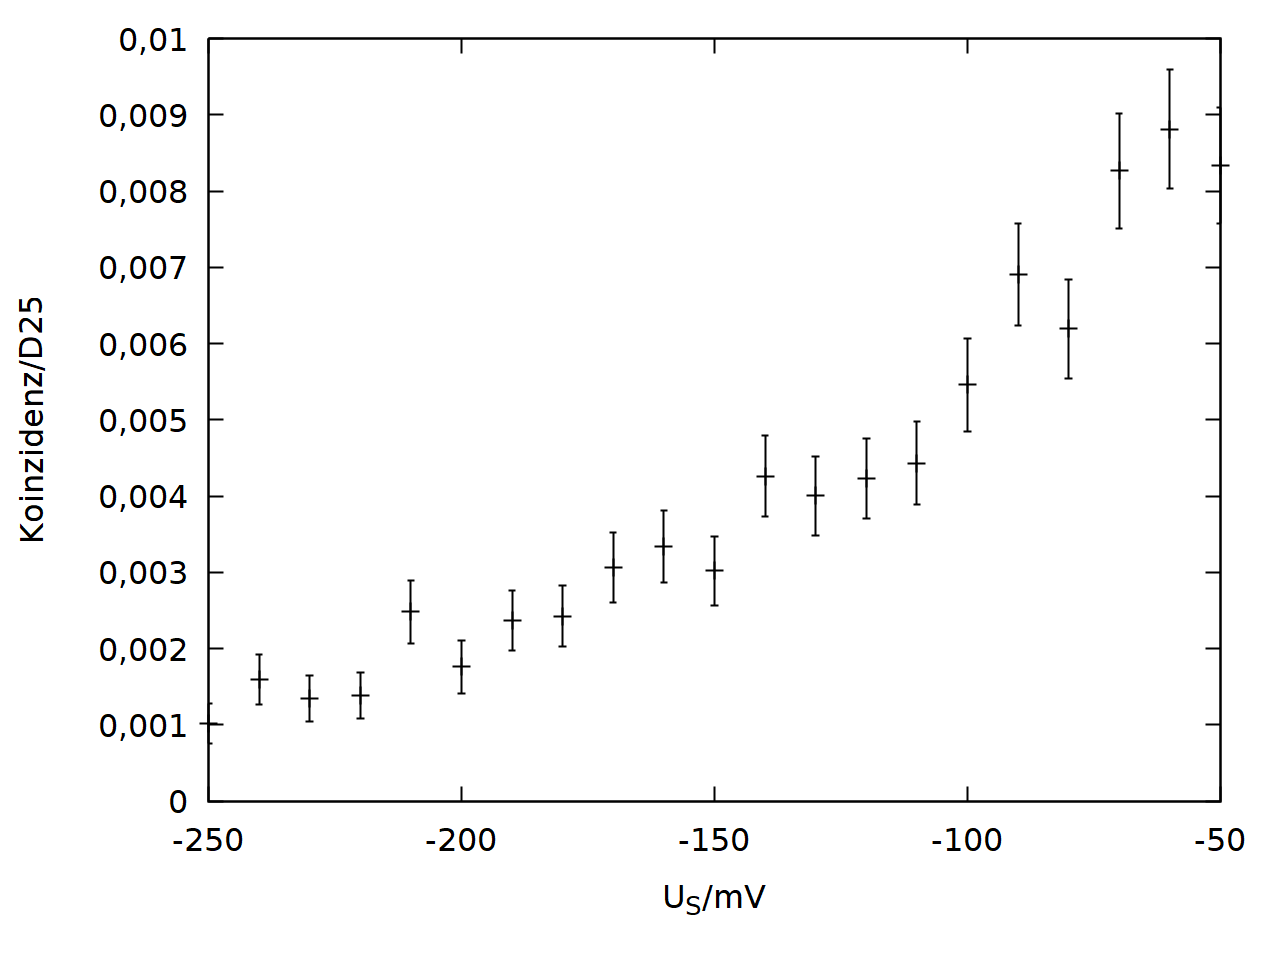
\includegraphics[width=0.75\linewidth]{data/friedrich/schwelle.png}
\caption{Koinzidenzen/D25 über der Schwellenspannung $U_S$}
\label{fig:schwelle}
\end{figure}
